\chapter{Arrays}
% Content for Chapter 7

\section*{Introduction}
An \textbf{array} is a collection of elements, all of the same type, stored in contiguous memory locations. It allows for efficient access using indices. Arrays can be \textit{static} (fixed size) or \textit{dynamic} (resized at runtime). In C++, the STL \texttt{vector} provides a dynamic array implementation.

\begin{figure}[h!]
  \centering
  \includegraphics[width=0.5\textwidth, height=5cm]{images/array.png}
  \caption{Conceptual representation of an array in memory}
  \label{fig:array_concept}
\end{figure}

\section{Array Declarations and Syntax}

\subsection*{1D Array Declaration}
\textbf{Static (C/C++):}
\begin{lstlisting}[caption=Static 1D Array Declaration]
int arr[5]; // Declares an array of 5 integers
\end{lstlisting}

\textbf{Dynamic (C++ using pointers):}
\begin{lstlisting}[caption=Dynamic 1D Array Declaration using Pointers]
int* arr = new int[5]; // Allocates memory for 5 integers dynamically
\end{lstlisting}

\textbf{Using STL Vector (C++):}
\begin{lstlisting}[caption=1D Array using STL Vector]
#include <vector>
vector<int> arr(5); // Vector of size 5
\end{lstlisting}

\subsection*{2D Array Declaration}
\textbf{Static (C/C++):}
\begin{lstlisting}[caption=Static 2D Array Declaration]
int matrix[3][4]; // 3 rows and 4 columns
\end{lstlisting}

\textbf{Dynamic (C++ using pointers):}
\begin{lstlisting}[caption=Dynamic 2D Array Declaration using Pointers]
int** matrix = new int*[3];
for(int i = 0; i < 3; i++) {
    matrix[i] = new int[4];
}
\end{lstlisting}

\textbf{Using STL Vector (C++):}
\begin{lstlisting}[caption=2D Array using STL Vector]
#include <vector>
vector<vector<int>> matrix(3, vector<int>(4)); // 3x4 2D vector
\end{lstlisting}

\subsection*{3D Array Declaration (Using STL Vector)}
\begin{lstlisting}[caption=3D Array using STL Vector]
#include <vector>
vector<vector<vector<int>>> arr3D(
    2, vector<vector<int>>(
           3, vector<int>(4)));
// 2x3x4 3D vector
\end{lstlisting}

\section{Time and Space Complexity}
\subsection*{Time Complexity}
\begin{itemize}
  \item \textbf{Access:} \(O(1)\) - Direct access via index.
  \item \textbf{Search:} \(O(n)\) - Linear search in the worst case.
  \item \textbf{Insertion/Deletion at End:} \(O(1)\) - Amortized time.
  \item \textbf{Insertion/Deletion at Beginning or Middle:} \(O(n)\) - Requires shifting elements.
\end{itemize}

\subsection*{Space Complexity}
\begin{itemize}
  \item \textbf{Space:} \(O(n)\) - Where \(n\) is the number of elements in the array.
\end{itemize}

\section{Memory Allocation and Address Calculation}

\subsection*{Memory Allocation}
Arrays are stored in contiguous memory locations. For an array declared as \texttt{int arr[n];}, the memory layout is illustrated below:

\begin{center}
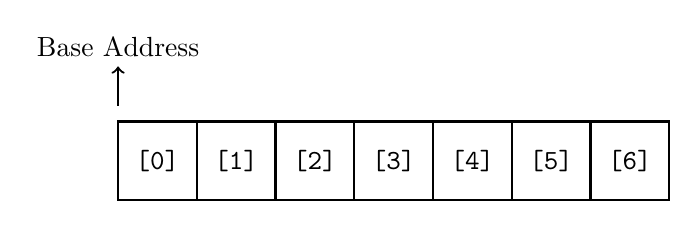
\begin{tikzpicture}[scale=1]
  \foreach \i in {0,1,2,3,4,5,6} {
    \draw[thick] (\i,0) rectangle (\i+1,1);
    \node at (\i+0.5,0.5) {\texttt{[\i]}};
  }
  \draw[->, thick] (0,1.2) -- (0,1.7) node[above]{Base Address};
\end{tikzpicture}
\end{center}

\subsection*{Address Calculation}
The address of the \(i\)th element is computed as:
\[
\text{Address of } arr[i] = \text{Base Address} + i \times \text{Size of each element}
\]

\subsection*{Indexing and Byte Addressing}
\textbf{0-Based Indexing:}
\[
\text{Address of } arr[i] = \text{Base Address} + i \times \text{Size}
\]
\textbf{1-Based Indexing:}
\[
\text{Address of } arr[i] = \text{Base Address} + (i-1) \times \text{Size}
\]

\section{Passing Arrays to Functions}
\subsection*{Example: Passing a 1D Array to a Function}
\begin{lstlisting}[style=cppstyle, caption=Passing Array to Function]
#include <bits/stdc++.h>
using namespace std;

void printArray(int arr[], int size) {
    for (int i = 0; i < size; ++i) {
        cout << arr[i] << " ";
    }
    cout << "\n";
}

int main() {
    int myArray[] = {10, 20, 30, 40, 50};
    int size = sizeof(myArray) / sizeof(myArray[0]);

    printArray(myArray, size);
    return 0;
}
\end{lstlisting}

\section{Two-Dimensional Arrays and Matrix Representation}
\subsection*{Row-Major Order}
The address of element \(A[i][j]\) is given by:
\[
\text{Address of } A[i][j] = B + [(i \cdot N) + j] \cdot w
\]
where \(B\) is the base address, \(N\) is the number of columns, and \(w\) is the size of each element.

\subsection*{Column-Major Order}
The address of element \(A[i][j]\) is:
\[
\text{Address of } A[i][j] = B + [(j \cdot M) + i] \cdot w
\]
where \(M\) is the number of rows.

\subsection*{Example: 2D Array in C++ (Row-Major Order)}
\begin{lstlisting}[style=cppstyle, caption=2D Array in Row-Major Order]
#include <bits/stdc++.h>
using namespace std;

int main() {
    int A[2][3] = {{1, 2, 3}, {4, 5, 6}};
    
    for (int i = 0; i < 2; i++) {
        for (int j = 0; j < 3; j++) {
            cout << A[i][j] << " ";
        }
        cout << endl;
    }
    return 0;
}
\end{lstlisting}

\section{Multidimensional Arrays}
Beyond 2D arrays, multidimensional arrays (such as 3D arrays) are used in applications like 3D graphics, simulations, and complex data representations.

\subsection*{Example: 3D Array (Using STL Vector in C++)}
\begin{lstlisting}[style=cppstyle, caption=3D Array Declaration using STL Vector]
#include <bits/stdc++.h>
using namespace std;

int main() {
    vector<vector<vector<int>>> arr3D(
        2, vector<vector<int>>(
               3, vector<int>(4, 0))); // 2x3x4 3D vector initialized with 0
    
    // Accessing an element:
    arr3D[0][1][2] = 42;
    
    cout << "Element at [0][1][2]: " << arr3D[0][1][2] << endl;
    return 0;
}
\end{lstlisting}

\section{Matrix Representation and Applications}
A matrix is typically represented as a 2D array and is used in:
\begin{itemize}
  \item Image representation (pixels)
  \item Graph adjacency matrices
  \item Dynamic programming tables
  \item Mathematical computations
\end{itemize}

\section{Drawbacks of Arrays}
Despite their efficiency, arrays have some limitations:
\begin{enumerate}
  \item \textbf{Fixed Size:} The size must be known at compile time for static arrays.
  \item \textbf{Memory Waste:} Overestimating size leads to unused memory, while underestimating can cause overflow.
  \item \textbf{Costly Insertions/Deletions:} Shifting elements results in \(O(n)\) time operations.
  \item \textbf{No Built-in Bound Checking:} Accessing out-of-bound indices causes undefined behavior.
  \item \textbf{Homogeneous Data:} Arrays store elements of the same type only.
  \item \textbf{Contiguous Memory Requirement:} Large blocks of contiguous memory might not be available in fragmented systems.
\end{enumerate}

\textbf{Solution:} Use STL containers like \texttt{vector} for dynamic arrays.

\section{Summary Table of Array Types and Syntax}
\begin{center}
\scriptsize % Or use \small if too tiny
\renewcommand{\arraystretch}{1.5}
\begin{tabular}{|l|p{3.2cm}|p{3.2cm}|p{4.5cm}|}
\hline
\textbf{Array Type} & \textbf{Declaration Syntax} & \textbf{Memory Allocation} & \textbf{Example / Notes} \\\hline

1D Static Array & \texttt{int arr[5];} & Stack, Contiguous & \texttt{int arr[5] = \{1, 2, 3, 4, 5\};} \\\hline

1D Dynamic Array & \texttt{int* arr = new int[5];} & Heap, Contiguous & Allocated at runtime using \texttt{new} \\\hline

2D Static Array & \texttt{int matrix[3][4];} & Stack, Row-major & 3 rows, 4 columns declared statically \\\hline

2D Dynamic Array & \texttt{int** matrix = new int*[3];} & Heap (row pointers), Contiguous rows & Allocate each row: \texttt{matrix[i] = new int[4];} \\\hline

STL 1D Vector & \texttt{vector<int> arr(5);} & Heap, Dynamic resizing & Uses STL; resizable, auto-managed memory \\\hline

STL 2D Vector & \texttt{vector<vector<int>> matrix;} & Heap, Nested Vectors & Allows jagged arrays; dynamic allocation \\\hline

STL 3D Vector & \texttt{vector<vector<..<int>.>} & Heap, Fully Dynamic & Example: \texttt{vector<vector<vector<int>>> arr3D(2, vector<vector<int>>(3, vector<int>(4)));} \\\hline
\end{tabular}
\captionof{table}{Summary of Array Types, Memory Allocation, and Syntax in C++}
\end{center}


\section{Additional Diagrams}
\subsection*{1D Array Memory Layout}
\begin{figure}[H]
\centering
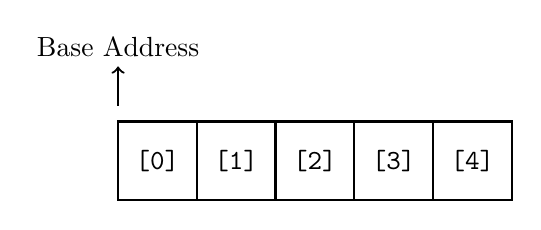
\begin{tikzpicture}[scale=1]
  \foreach \i in {0,1,2,3,4} {
    \draw[thick] (\i, 0) rectangle (\i+1, 1);
    \node at (\i+0.5,0.5) {\texttt{[\i]}};
  }
  \draw[->, thick] (0,1.2) -- (0,1.7) node[above]{Base Address};
\end{tikzpicture}
\caption{Memory layout of a 1D array with 5 elements.}
\end{figure}

\subsection*{2D Array Memory Layout (Row-Major)}
\begin{figure}[H]
\centering
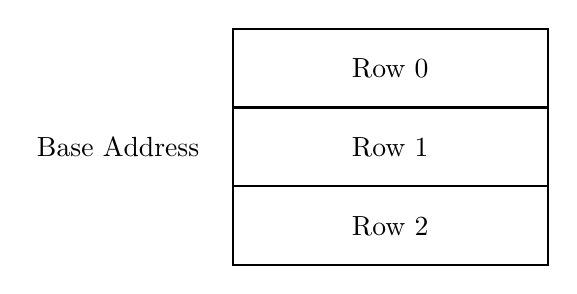
\begin{tikzpicture}[scale=1]
  \draw[thick] (0,0) rectangle (4,1) node[midway]{Row 0};
  \draw[thick] (0,-1) rectangle (4,0) node[midway]{Row 1};
  \draw[thick] (0,-2) rectangle (4,-1) node[midway]{Row 2};
  \node[anchor=east] at (-0.3,-0.5) {Base Address};
\end{tikzpicture}
\caption{Row-major layout of a 2D array (3 rows, 4 columns).}
\end{figure}


\section{Index Diagram and Table}

Consider a 1D array with 5 elements. The following table and diagram illustrate how array indices correspond to the stored elements.

\subsection*{Index Mapping Table}
\begin{table}[H]
\centering
\begin{tabular}{|c|c|}
\hline
\textbf{Index} & \textbf{Element (Label)} \\\hline
0 & \texttt{arr[0]} \\\hline
1 & \texttt{arr[1]} \\\hline
2 & \texttt{arr[2]} \\\hline
3 & \texttt{arr[3]} \\\hline
4 & \texttt{arr[4]} \\\hline
\end{tabular}
\caption{Mapping of indices to array elements for a 1D array}
\end{table}


\subsection*{1D Array Index Diagram}
\begin{figure}[H]
\centering
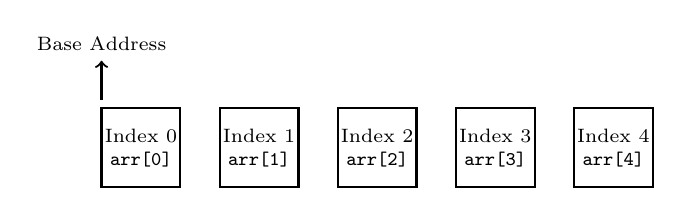
\begin{tikzpicture}[scale=1, every node/.style={font=\scriptsize}]
  % Draw boxes for each element
  \foreach \i in {0,1,2,3,4} {
    \draw[thick] (\i*1.5,0) rectangle (\i*1.5+1,1);
    \node at (\i*1.5+0.5,0.65) {Index \(\i\)};
    \node at (\i*1.5+0.5,0.35) {\texttt{arr[\i]}};
  }
  % Draw Base Address arrow
  \draw[->, thick] (0,1.1) -- (0,1.6) node[above]{Base Address};
\end{tikzpicture}

\caption{Index diagram for a 1D array of 5 elements}
\end{figure}


